\section{Alternative Models}
\label{sec:evaluation-alternative-models}
\todo[author=Kasper]{Endnu ikke skrevet}

When seeing the results of the user test presented in \cref{sec:evaluation:user-tests} and finding that the accuracy of the system is roughly 44\%, i.e. the correct action is triggered in 44\% of the cases, we started considering if alternative models for the context engine would be better suited or if improvements to the current model would address the issues.

\subsection{Influence Diagram}

Influence diagrams can be regarded as Bayesian networks extended with decision variables and utility functions \cite{kjaerulff2008bayesian}. \Cref{fig:evaluation:alternative-models:influence-diagram} shows an influence diagram modelling a context engine. The model does not correspond exactly with the model previously presented in this report but is an alternative model.

We will not go into details about influence diagrams in this report. As for the graphical representation of an inflence diagram, the square nodes represent \emph{decision nodes}, i.e. something we must decide to do or not to do. Rhombe nodes represent \emph{utility nodes} describing a \emph{utility function}. In an influence diagram we are generally interested in taking the decision that results in the highest utility, therefore utility can be regarded a measurement of the quality of a decision.

In the model presented in \cref{fig:evaluation:alternative-models:influence-diagram}, the utility is a function of the gesture, room and action. We assign a high utility to combinations of gesture and room that are part of a gesture configuration. 

Influence diagrams provide a natural way of including the system state, as actions which it does nto make sense to trigger given the current state of the system, can be assigned a very low utility.

\begin{figure}[!h]
\centering
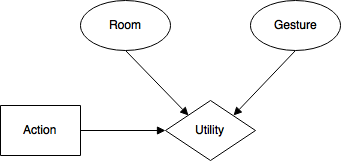
\includegraphics[width=0.50\textwidth]{images/influence-diagram}
\caption{Example model of the context engine using an influence diagram.}
\label{fig:evaluation:alternative-models:influence-diagram}
\end{figure}

Due to inference in the probabilistic network, actions are assigned a utility when we have soft or hard evidence on the gesture and room nodes. The utility of an action is shown with dark green bars below the name of the action in \cref{fig:evaluation:alternative-models:hugin-influence-diagram}. For example, the utility of the \emph{Shelves\_Lamp\_Toggle} is 6682, making it the action with the highest utility and thus the action we decide to trigger\footnote{More information on influence diagrams in Hugin is available at \url{http://www.hugin.com/technology/getting-started/ids}}.

The scenario previously discussed in \cref{sec:evaluation:user-tests} in which an incorrect action was triggered because a gesture is associated with multiple actions and thus those actions get a belief is shown in an influence diagram in \cref{fig:evaluation:alternative-models:hugin-influence-diagram}. In contrast to the model based on a Bayesian network, the correct action can be triggered with greater confidence when utilizing the influence diagram.

When testing the Bayesian network with a subset of the recorded data during the user tests, we found that when using the influence diagram, we were able to more often trigger the correct action. During the user test, participant 7 a correct action was triggered 36\% of the time. Using the exact same beliefs on gesture and room nodes in the influence diagram, the correct action is triggered 50\% of the time.

% Note that during the tests with the Bayesian network we considered the outcome of performing an action acceptable if a list of suggested actions were shown and the intended action was in the list. This was not taken into account when testing the influence diagram with the data from participant 7 and as such the accuracy of the influence diagram may increase if a threshold for the utility of accepted actions is introduced.

\begin{figure}[h]
\centering
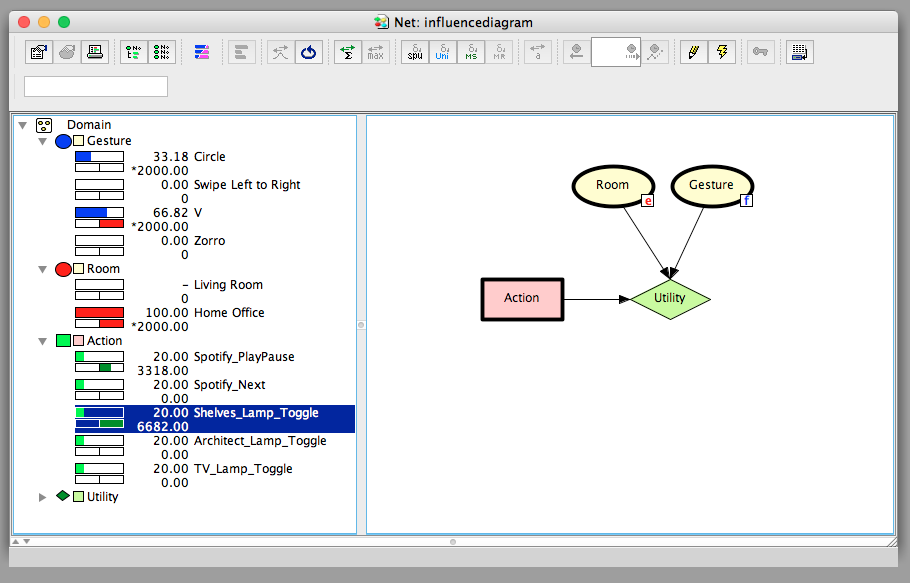
\includegraphics[width=\textwidth]{images/hugin-influence-diagram}
\caption{Screenshot of example influence diagram in Hugin. The screenshot shows that the influence diagram solves the problem of a single gesture being bound to multiple actions, can result in an incorrect action being triggered because the belief is reduced as shown in \cref{table:participant-2-first-run} and discussed in \cref{sec:evaluation:user-tests}.}
\label{fig:evaluation:alternative-models:hugin-influence-diagram}
\end{figure}


%%% Local Variables:
%%% mode: latex
%%% TeX-master: "../../master"
%%% End:
